\documentclass[a4paper,11pt,notitlepage]{report}

\usepackage[utf8]{inputenc}
\usepackage{amsmath}
\usepackage{listings}
\usepackage[hidelinks]{hyperref}
\usepackage{catoptions}
\usepackage[left=0.8in, right=0.8in, top=0.8in, bottom=0.8in]{geometry}
\usepackage{color}
\usepackage{soul}
\usepackage{float}
\usepackage{framed}
\usepackage[sc]{mathpazo}
\linespread{1.20}         % Palatino needs more leading (space between lines)
\usepackage[T1]{fontenc}
\usepackage{microtype}
\usepackage{enumerate}
\usepackage{courier}
\usepackage{graphicx}
\usepackage{enumitem}
\usepackage{lipsum}
\usepackage{tikz}
\usepackage{caption}
\usepackage{subcaption}
\usepackage{verbatim}
\usetikzlibrary{shapes,arrows}
\usepackage{wrapfig}

\graphicspath{ {./Images/} }

\pdfinfo{
  /Title    (Building Serious Games - Design4Health)
  /Author   (Ralf Nieuwenhuizen, David Prihoda, Ismini Psuxoula, Arnold Schutter, Shen Shuheng)
  /Creator  (Ralf Nieuwenhuizen, David Prihoda, Ismini Psuxoula, Arnold Schutter, Shen Shuheng)
  /Producer (Ralf Nieuwenhuizen, David Prihoda, Ismini Psuxoula, Arnold Schutter, Shen Shuheng)
  /Subject  (Building Serious Games)
}

% Settings for hyperref package (e.g. wat \autoref en \nameref moeten doen)
\hypersetup{
  colorlinks  = false,
  linkcolor   = [rgb]{0.1,0.1,0.5},
  citecolor   = [rgb]{0.5,0.1,0.1},
  filecolor   = [rgb]{0.1,0.5,0.5},
  urlcolor    = [rgb]{0.1,0.1,0.7}
}

\newcommand{\todo}[1] {\hl{#1}}
\setlength{\parindent}{0cm}

\begin{document}

% Define block styles
\tikzstyle{block} = [rectangle, draw, fill=white!20, 
    text width=7em, text centered, rounded corners, minimum height=4em]
\tikzstyle{blockSmall} = [rectangle, draw, fill=white!20, 
    text width=4em, text centered, rounded corners, minimum height=3em]
\tikzstyle{line} = [draw, -latex']
		
\begin{center}
\vskip 1cm
{\Huge Design4Health \vskip 2mm}
{\Large IN4302TU -- Building Serious Games \vskip 1cm}
{\Huge Game Design \vskip 1cm}

\begin{tabular}{ l l }
\textbf{Ralf Nieuwenhuizen} & ($4080408$) \\
\textbf{David Prihoda} & ($4405951$) \\
\textbf{Ismini Psychoula} & ($4411285$) \\ 
\textbf{Arnold Schutter} & ($4260724$) \\ 
\textbf{Shuheng Shen} & ($4298225$)
\end{tabular} 

\end{center}

%\newpage
%\tableofcontents
%\newpage

\chapter{Game Design}

\section{Introduction}
We propose a game which encourages the user to regularly perform different types of physiotherapy exercises in order to stay healthy by representing his progress in the storyline. The user’s intrinsic motivation to stay healthy is supported by educating him about the impact different exercises have on his body and by an engaging interaction using smartphone sensors. The user is provided with feedback on the number and type of exercises he has performed and their impact on his different body regions. 

\section{Game design}

\subsection{Real-life implications}
From the real-life point of view, the user is encouraged to perform isolated exercises that are carefully selected to cover all body regions. He is also able to set his own personal goals by choosing to perform sets of exercises focused on a specific body region. During the execution of the exercise, a smartphone is used to measure the movements and to provide acoustic feedback. Moreover, the game reflects the user’s long-term progress, encouraging him to continue exercising regularly throughout the day and also to focus on all different body regions equally. All the real-life implications of performing the exercises are explicitly mentioned in the game, while being seamlessly incorporated in the storyline.

\subsection{Game Story}
The game starts with a story. 
\\
\begin{wrapfigure}{l}{150px}
  \vspace{-30pt}
	\begin{center}
		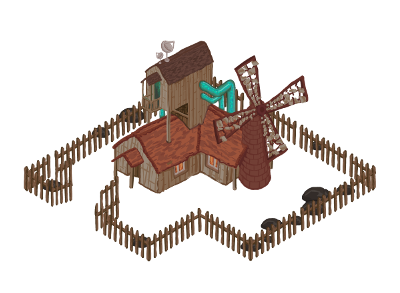
\includegraphics[width=150px]{Images/farm.png}
	\end{center}
  \vspace{-30pt}
	\caption{The farm}
  \vspace{-20pt}
	\label{fig:farm}
\end{wrapfigure}
\textit{2542 AD. Your uncle was one of the first people to buy land in an unknown planet and decided to turn it into a farm to facilitate the earth’s growing needs of foods. As years went by the farm became very profitable and produced the most sought out products. You were very surprised when you received a mail saying that your uncle had left you the farm years ago but you only heard of it now. After so many years, the fields on planet Yeo are unused and empty. Will you be able to salvage the farm? Spend your money wisely to grow the company and unlock new possibilities by doing the exercises.}

\subsection{Gameplay}
The user, a novice farmer, is instructed by a virtual physiotherapist, an old farmer, to learn and perform regularly different types of exercises that help him stay healthy in real life and progress in the game. By growing crops and breeding livestock the hero can become a more skilled farmer and revive the company. 
\\\\
The game mechanics are shown in Figure~\ref{fig:gameconcept}. The central point is the exercise, which powers all the progress in the game. 

\begin{figure}[h]
	\centering
		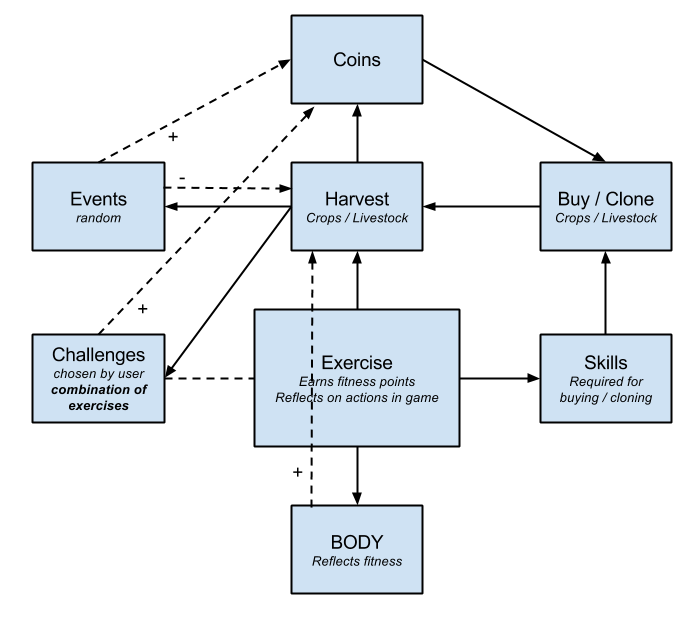
\includegraphics[width=0.80\textwidth]{Images/gameconcept.png}
	\vspace{-15pt}
	\caption{Game mechanics}
	\label{fig:gameconcept}
\end{figure}

To grow crops or breed animals on the farm, the farmer has to learn skills and earn coins. Skills are learned by performing specific exercises in real-life. After learning a skill, the farmer can pay coins to buy the corresponding crops or livestock and place them on tiles in the map. In a certain time interval the crops are ripe and can be harvested and livestock products can be gathered, this requires specific exercises to be executed in real-life. 
\\\\
The user starts with a small amount of coins that allows him to buy the first crops. Coins can be earned by selling the products on the market, extra coins are earned by using specific batches of products to complete challenges and events. Challenges consist of a story and requires the execution of a set of exercises focused on a specific body region. Events are random challenges that bring the surprise element into the game.
\\\\
The farmer is equipped with a Bionic Outer Dimension Yeosuit, or BODY, in short, which reflects all the exercises the user has performed in the game. For example, after performing ten exercises that focus on shoulder muscles, the BODY will automatically get a visible upgrade. This way, the user is informed which body regions he has improved and which need to be focused on in the future.

\subsection{Example game scenario}
This section provides an example of the game play. In this example, the user learns the skill of growing apple trees by performing the exercise to pick them (stretching his middle back and shoulders by alternating arms, reaching one as high as he can and as low as he can, while standing upright with his back to the wall). After a satisfactory execution of the exercise, he is able to buy apple trees with his money and plant them on any available tile on the map. After a few hours, the user will get a notification that the apples can be harvested. To harvest them, the user has to perform an exercise of picking apples . After the apples are harvested, the user can either sell them for coins directly, or store different crops to complete a challenge for extra money. The completion of a challenge requires a certain amount of crops, but also new exercises specific for a certain body part. 

\section{Game features}
In the sections below there is an extended description of all the game features and their specifications. The sections with a star are planned for the final version of the game, however they will not be included in the first playable. 

\subsection{The overview}
At the start of the game, the introducing story will be presented to the player before the farm is shown. A short explanation of the game will be given, and then the player is ready to start his adventure.

By clicking on the farm, the user can see his current inventory of items. (see figure~\ref{fig:sketch-overview})

\begin{figure}[h]
	\centering
		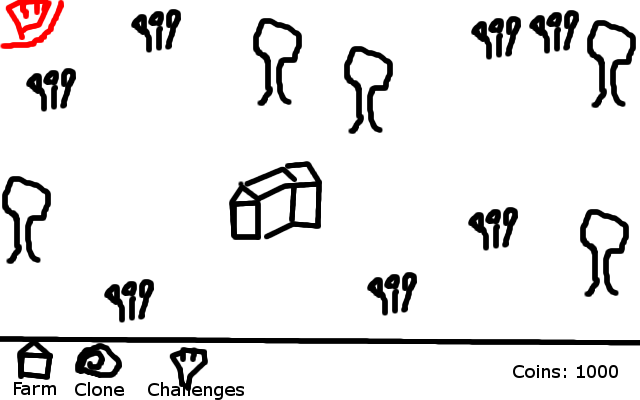
\includegraphics[width=0.60\textwidth]{Images/sketch-overview.png}
	\caption{Sketch of the overview of the game, with menu items}
	\label{fig:sketch-overview}
\end{figure}

\subsection{Mentor Phil}
Once you get to the farm, you discover there is a very old friend of your uncle's, Phil, who is around 60 years old, but still very much in shape. He will serve as your mentor and "physiotherapist" in the game. Phil explains the purpose and correct execution of each exercise to you. During the game, the mentor and the player will become friends.

\subsection{The farmer}
In the game, the player will be impersonated by a farmer. This farmer will perform all the tasks on the screen the player performs in real-life. The farmer wears a BODY which is upgraded according to performed exercises.

\subsection{BODY}
Apart from the advice part that the player gets from the mentor, he also gets reflection of his progress in the game in the form of a "BODY". The player has a list of points, one for each body part (arms, legs, abs, back), and each executed exercise will yield some points for a specific body part. When the points for a certain bodypart have reached a certain amount, the player will be awarded an upgrade to his BODY. This way, the player will be warned if he's focussing too much on one or several body parts, and he will be motivated to also focus on the other parts. The player has a free choice in the exercises he performs, but is motivated to make a balanced scheme. 
\\\\
The level of the player is defined by the progress of the BODY. In this way, the BODY gives an indication of the progress in the game and the physical performance. The level is defined by the lowest level of the body parts (a chain is as strong as its weakest link). A higher level gives the player more skills and unlocks new crops and livestock.

\subsection{Exercises}
During the game, players will be confronted with several exercises, which they will have to perform in real life. These exercises will allow them to either plant or harvest a crop, or to perform a task, like milking the milkatrons. Prior to each exercise a clear explanation is shown about the movement the player has to perform demonstrated by a drawing of the mentor. The phone is used to measure the execution of the exercise and should be held by the player. The accelerometer of the phone measures the movement.
\\\\
A sketch of what an exercise will look like is shown in Figure~\ref{fig:sketch-exercise}.

\begin{figure}[h]
	\centering
		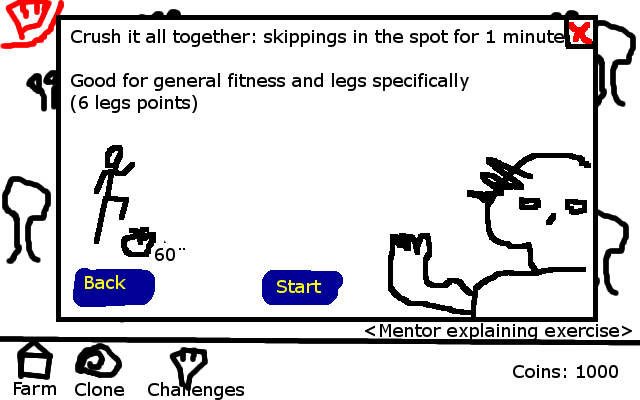
\includegraphics[width=0.60\textwidth]{Images/sketch-exercise.png}
	\caption{Sketch of the exercise view}
	\label{fig:sketch-exercise}
\end{figure}

\subsubsection{List of exercises}
\begin{enumerate}
\item “Apple picking” - Harvesting apples
\begin{itemize}
\item Start from standing up straight
\item Raise one arm (with the phone in hand) as high as you can, while you raise your opposite knee until you have a 90 degrees angle both between legs and core and between upper and lower leg
\item Finally, try to keep this stance while standing on your toes
\item Repeat on the other side (switch the phone hand!)
\end{itemize}
\item “Arm Circles” - Harvesting wheat
\begin{itemize}
\item Stand up and extend your arms straight out by the sides. The arms should be parallel to the floor and perpendicular to your torso.
\item Slowly start to make circles of about 1 foot in diameter with each outstretched arm. Breathe normally as you perform the movement.
\item Continue the circular motion of the outstretched arms for about ten seconds.
\item Then reverse the movement, going the opposite direction.
\end{itemize}
\item “Rocket jumps” - Crushing things together
\begin{itemize}
\item Keep your phone in two hands
\item Begin in a relaxed stance with your feet shoulder width apart and hold your arms close to the body
\item To initiate the move, squat down halfway and jump back up as high as possible
\item Fully extend your entire body, reaching overhead as far as possible. As you land, absorb your impact through the legs
\item Repeat x times
\end{itemize}
\end{enumerate}
\subsection{Challenges}
The player will have a list of challenges from which he can at anytime pick one and execute that to receive bonus coins. These challenges have an underlying set of exercises that can either be focused on one body part, or they can be a complete body workout. The mentor will explain about that. Challenges are proposed to the player as an appealing task in the game, for example to make a spaceapple pie for your neighbouring Yeowoman that is ill. The player would have to perform some exercises that would be needed to get the ingredients for the spacepie, and by doing that he would have completed a workout without noticing. The mentor will inform the player of that afterwards, to raise awareness.
\\\\
A sketch of what an active challenge will look like is shown in Figure~\ref{fig:sketch-challenge}.

\begin{figure}[h]
	\centering
		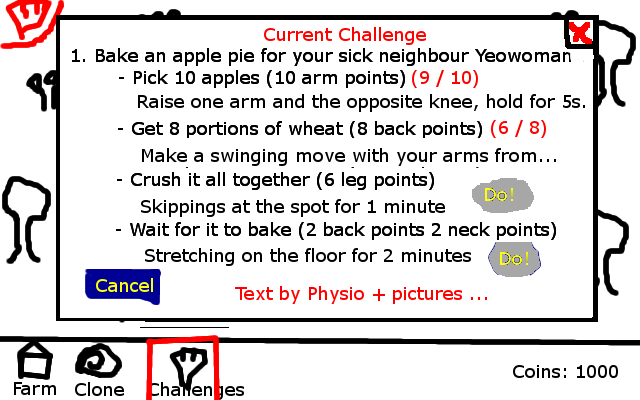
\includegraphics[width=0.60\textwidth]{Images/sketch-challenge.png}
	\caption{Sketch of current challenges view}
	\label{fig:sketch-challenge}
\end{figure}

\subsubsection{Example challenges}
\begin{enumerate}
\item Bake a spaceapple pie for your sick neighbour Yeowoman. (Full-body)
\begin{itemize}
\item Pick 10 apples (arms) - See exercise “Apple picking”
\item Get 8 portions of wheat (back) - See exercise “Arm circles”
\item Crush it all together (legs) - See exercise “Rocket jumps”
\end{itemize}
\item Make a wool doll for your cousin as a birthday present. (Back)
No exercises specified yet
\end{enumerate}
\subsection{Events}
Events will occur randomly in the game and are used to create extra challenges for the player. An example of an event is a raid of Space Cowboy to the farm or a disease that comes to your planet. More severe events will happen once the player has reached a higher level. The chances of getting events will decrease when the player is active.
\subsubsection{List of events}
\begin{itemize}
\item Save the farm from an attack of space cowboys
\item Save your crops from the Pest
\item Save the farm from an attack of neighbouring Aliens
\end{itemize}
\subsection{Money}
When the game begins the player is given a 1000 coins to start developing his farm. After that first allowance he can earn more money by selling his products on the market.
\subsection{Growing crops}
Each type of crop has a name, a cost, a revenue that it brings in when harvested, the time it takes for it to grow. Plants will only last one harvest and have to be harvested soon enough (e.g. two times its growth time), or they die. Trees can last multiple harvests.
\\\\
A sketch of what the clone view will look like is shown in Figure~\ref{fig:sketch-clone}.

\begin{figure}[h]
	\centering
		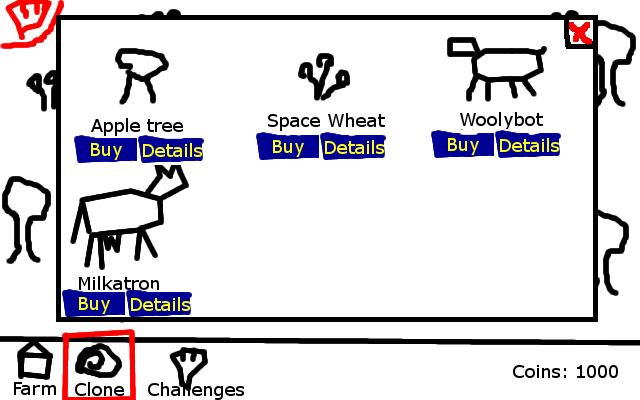
\includegraphics[width=0.60\textwidth]{Images/sketch-clone.png}
	\caption{Sketch of cloning crops / livestock}
	\label{fig:sketch-clone}
\end{figure}

\subsubsection{List of crops (cost, time to grow [minutes], revenue of single harvest, number of harvests)}
\begin{itemize}
\item Spacewheat (5, 1, 10, 1)
\item Tomatoid plant (30, 3, 50, 1)
\item Sprice plant (50, 10, 50, 1)
\item Yeotato plant (60, 15, 100, 1)
\item Yeogrenade plant (100, 30, 200, 1)
\item Zorganic melon plant (300, 240, 750, 1)
\item Spaceapple tree (100, 600, 75, 5)
\end{itemize}

The amount of space around the farm is fixed throughout the duration of the game. While the game progresses, some old crops or livestock might be sold to free space for new options.
\subsection{Cloning livestock}
Each type of livestock has a name, a cost, a revenue it brings when exploited and the time it takes for it to be ready (for example milking a Milkatron every 8 hours will produce 2 buckets of milk that can be sold for 40 coins each).

\subsubsection{List of livestock (cost, time to grow [minutes], revenue of single exploitation)}
\begin{itemize}
\item Polychick (15, 5, 10 (2 eggs))
\item Metagoat (30, 30, 10 (1 milk))
\item Milkatron (100, 240, 40 (4 milk))
\item Woolybot (100, 600, 30 (2 balls of wool))
\item Piggium (200, 1440, 50 (1 meat))
\item iBeef (300, 2880, 150 (3 meat))
\item Unicorn (1000, 4320, 1000 (1 magical hair))
\end{itemize}
\subsection{Market}
From the farm you are able to see your inventory. Here you will have an overview of all the items you currently possess. These items can be sold on the market, giving you the revenue they are worth.
\\\\
A sketch of what the inventory will look like is shown in Figure~\ref{fig:sketch-inventory}.

\begin{figure}[h]
	\centering
		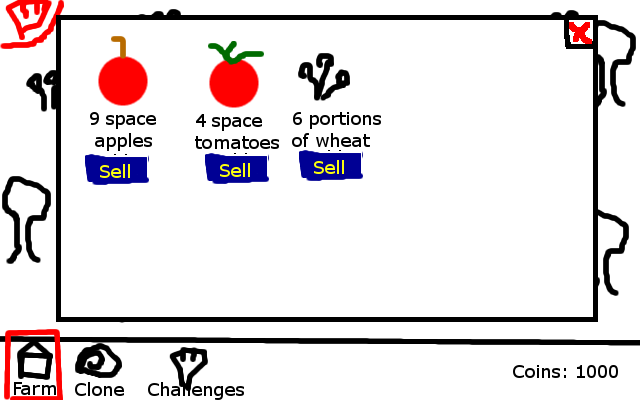
\includegraphics[width=0.60\textwidth]{Images/sketch-inventory.png}
	\caption{Sketch of the inventory}
	\label{fig:sketch-inventory}
\end{figure}

\section{Phases}
This section shows the planning for the project. An overview is given for each phase about what part of the game should be completed. 
\subsection{Designing the game}
Before starting on developing the actual software, there will be sketches for all screens of the game, to create a clickable static prototype. This will be presented to the group, a final decisions about the design is made after this session in week 2.
\subsection{First playable}
The first playable will be a small version of the final game. It will not be complete, but the vital functionalities will be completed. In this phase a basic version of the game is available to be played and some exercises can be performed. Some user tests will be done and the progress will be reported to the commissioners.
\subsubsection{Week 3}
\begin{itemize}
\item Map view (farm and fields) is functional
\begin{itemize}
\item Farm and fields are showed on the screen with right dimensions
\item Fields are clickable for harvest and planting
\end{itemize}
\item Panning is possible through screen
\item Rotation of the screen to landscape
\item Currency is implemented
\item Three screens are completed and functional
\begin{itemize}
\item Clone: Crops can be cloned and the action is connected with currency
\item Map: Crops can be planted, harvested and show progress
\item Exercise: Screen shows and explains the exercise to be done to complete a task
\end{itemize}
\item Accelerometer is connected to the software and is able to distinguish if movement was performed
\end{itemize}
\subsubsection{Week 4}
\begin{itemize}
\item Two crops are fully functional in-game
\item Three exercises are fully functional in-game
\begin{itemize}
\item Accelerometer measures correct execution of exercise
\end{itemize}
\item Test
\begin{itemize}
\item Game play: The game works fluently and correct
\item Intuitiveness: Navigation through screens and action buttons are intuitive 
\end{itemize}
\end{itemize}
\subsection{Beta version}
The beta version will already have all of the main features of the final game. Most of the crops and livestock will be buildable and the game works fluently. The beta version will be tested on the target audience.
\subsubsection{Week 5}
\begin{itemize}
\item Livestock is implemented in the game
\item Two extra screens are functional
\begin{itemize}
\item Challenge screen: Challenges can be selected and executed
\item Farm screen: The amount of harvested crops and completed products are shown
\end{itemize}
\item The view is scalable
\item Complete the functionalities of the gameplay
\begin{itemize} 
\item Currency
\item Exercises with detailed descriptions and measurements (>10) 
\item Challenges (>5)
\item Events (>2)
\end{itemize}
\item Design models for
\begin{itemize}
\item Mentor Phil
\item Crops (>5)
\item Livestock (>5)
\end{itemize}
\item Test 
\begin{itemize}
\item Story: Purpose of the game and actions to be taken are clear 
\item Intuitiveness: Navigation through screens and action buttons are intuitive
\item Game play: The game works fluently and correct
\item Features: Are there more wishes for features
\end{itemize}
\end{itemize}
\subsubsection{Week 6}
\begin{itemize}
\item Sounds are added for the exercises
\item Sounds are added to the game
\item The BODY with different levels is designed and implemented
\item Completed the exercise-related functionalities of the gameplay
\begin{itemize} 
\item Exercises with detailed descriptions and measurements (>15) 
\item Challenges (>10)
\item Events (>4)
\end{itemize}
\item Implemented comments from previous user tests
\item Tested:
\begin{itemize}
\item Game play / Features
\item Exercises: Opinion about exercises and willingness to do them
\end{itemize}
\end{itemize}
\subsection{Final version}
In the final version all the features are added from the list above. The game will be tested again on the target audience and the gameplay is improved.
\subsubsection{Week 7}
\begin{itemize}
\item Improve game (according to user tests)
\item Test
\begin{itemize}
\item Gameplay: Engagement of the user in the game
\item Features: Are there more wishful features
\end{itemize}
\item Fix bugs
\end{itemize}
\subsubsection{Week 8}
\begin{itemize}
\item Final user tests
\item Final report
\end{itemize}

\section{Testing plan}
In order to check the usability of our game. We will evaluate it in the form of questionnaires. As for the effectiveness of some specific modules, an A-B test for the final version will also be conducted following the between-subjects design if necessary.

\subsection{Experiment Setting}
\subsubsection{Participants}
The subjects of the testing will be adults between the ages 18-30. We aim for sufficient people for each phase.
\subsubsection{Materials}
\begin{itemize}
\item Informed consent form
\item A room for the experiment
\item Questionnaires for the participants
\item Smartphones with our game installed
\end{itemize}
\subsubsection{Experiment Procedure}
\begin{itemize}
\item The participants enter the room.
\item We will give a brief introduction of our game to the participants.
\item They will be requested to play the game  and focus on the aspects we want to test each time. During this section we will ask the test persons to speak out loud and if they agree we will film them. This way we can get the most out of the test session.
\item After the gaming session is finished, the participants will have to answer the questionnaire.
\end{itemize}
\subsubsection{Questionnaire}
This is the general model of the questionnaire which will be specified accordingly depending on which components of the game we want to test each time.
%ToDo: might will have to be modified later wrt the prototype
\begin{itemize}
\item Sex? male/female
\item Age? 18-25, 25-30, over 30
\item Have you ever played a similar game like this? Yes/No
\item If so, what is the name of that game?
\item Do you think the challenge was hard to finish? Likert Scale: “easy”(1) ~ “hard”(7)
\item Is the process of fulfilling the task clear?  (i.e., Are you fully aware of what could be the next step?)  Likert Scale:  “I have no idea”(1) ~ “I have a clear idea”(7)
\item Was the drawing demonstrating the exercise clear? Likert Scale:  “I couldn’t understand what movements the illustrations represented”(1) ~ “The demonstration was clear.”(7)
\item Does the smartphone sense your movement well?   Likert Scale: “The sensors couldn’t sense my movement at all.”(1) ~ “The sensors work well.”(7)
\item Did the game react fast enough on your actions?  Likert Scale: “It was too slow.”(1) ~ “It was too fast.”(7)
\item Do you think this game can help you relax and prevent you from sitting on the chair the whole day? Likert Scale: “No, I don’t think so.”(1) ~ “Yes, I totally agree.”(7)
\item Were the graphics visually appealing?  Likert Scale: “I didn’t like them at all.”(1) ~ “I liked them very much.”(7)
\item Was the text used in description clear and understandable? yes/no [comments section]
\item The pace of the game is  Likert Scale: “Too slow.”(1) ~ “Too fast.”(7)
\item The aim of the game is …: Likert Scale: “rather confusing”(1) ~ “clear”(7)
\item Free comments section
\end{itemize}
					
\section{Requirements}
\subsection{Meeting the requirements from the commissioners}
During the first meeting with the commissioners the requirements for the game were discussed.  From this session it seemed not to be important to focus specifically on physiotherapists and their patients. The focus is more on the use of sensors to keep people activate and motivate them to move. After this session we have decided not to focus too much on the physiotherapeutic part of the game, but more towards the activating nature of it.
\\\\
\textbf{The main goal of the project is: Explore the ways sensor technology can improve communication/engagement in an e-health environment. Inspire long-term self-management and sticking to self-imposed goals and lifestyle changes through digital means}. To support this goal we are using the sensors in mobile phones to measure exercises the player does in the game. By providing feedback to the users about their progress in fitness level (by the BODY) and the feedback per exercise about what body parts are trained by this exercise, and by the addicting nature of the game, it inspires a lasting lifestyle change in a positive way. The game can teach the user to use random previously not-utilised times during the day (e.g. performing squats while waiting for toast) to get their exercises done and reward them appropriately. This all serves the goal to change their habits. Driving lasting change.
\\\\
\textbf{Considering sub-goal 1: Raise patient’s awareness and sense of responsibility for their own health in an engaging way.}
The patient should be more focused on the exercises than on the farm itself. Therefore we have decided to think of the game more with the focus on the exercises. We will make a list of exercises categorized by bodyparts. These exercises are mapped to several actions in the game, instead of the other way around. In this way, it will  be easy to provide feedback to the user about what exercises he has done and what purpose this serves in real life (the feedback part is really important). Specific exercises for certain bodyparts could eventually be added and provided to users by adding new challenges.
\\\\
\textbf{Considering sub-goal 2: Enhance the feeling of being a team with your physiotherapist.}
To support the second subgoal, we have decided that once you get to the farm, you discover there is a very old friend of your uncle's, who is around 60 years old, but still very much in shape. He will serve as your mentor and "physiotherapist" in the game, so he will explain the purpose and correct execution of each exercise to you.

\subsection{Target audience}
The envisioned design will fulfill the requirement of being an engaging, activating game. This is all meant to activate people while doing an activity they love, gaming. The game will focus on young adults, as these are the people mostly concerned with exercise and activity. These people are also the ones who are most likely to make lifestyle changes. The game will be serious, as there is a clear purpose behind it of activating people and making them change to an active lifestyle, and it will be fun, as is proven by previous games in which you build up your own world, and have to show dedication to keep it up and running.
\subsection{Resources}
To derive a full up and running game from a paper prototype some resources will be needed. Because it will be a smartphone application, no external sensors will be needed at first. Plenty of open source software is available to fulfill our needs. The only cost we have is the Android Developer registration fee which is \$25.
\subsubsection{Hardware}
The only requirement for someone to play our game will be the possession of a smartphone. Several sensors on smartphones to measure the execution of exercises will be investigated. Most likely these will include the accelerometer, GPS, and microphone.
\subsubsection{Software}
The game will be developed for Android mobile phones, using open source software. 
We will do this using HTML5 supported by javascript, supported by LimeJS, and maybe more libraries. The HTML5 can be converted to a native app by using PhoneGap (\url{http://phonegap.com/}). This also gives us the option to convert to other mobile platforms, like iOS and Windows Phone



%\bibliography{synopsis}
%\bibliographystyle{plain}

\end{document}
